\section{Phase Two: Classification}\label{sec:eval_phase2} %This is where we examine if we can classify correctly
When using the created map, our aim is to determine if the system can sufficiently distinguish whether a receiving device is situated inside or outside the room.
To do this, we want to establish how well different devices can utilize the map to classify the device as \textit{inside} or \textit{outside}. 
\begin{figure}[h]
    \centering
    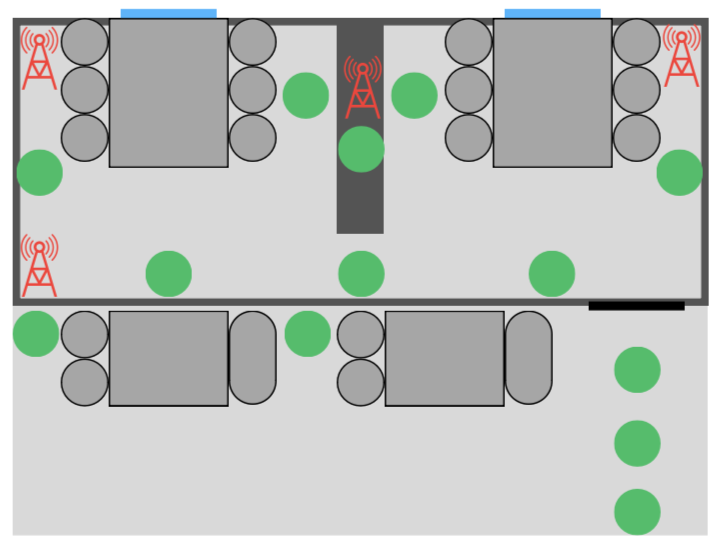
\includegraphics[scale=0.5]{images/experiment_setup.png}
    \caption{A sketch of the meeting room in which the experiments were carried out, decorated with beacon placements (red antenna) and measurement locations(green circles)}
    \label{fig:experiment_setup}
\end{figure}

As described in Section \ref{sec:bluetooth_low_energy}, physical obstacles can cause fluctuations in the received signals. 
Therefore, we design expirement such that classifcation measurements are taken in areas where some, none, and all of the beacons are blocked by physical obstacles. 
We perform measurements in the \textit{classification points}:
\begin{itemize}
    \item Along the walls inside of the meeting room, to examine border values of the map while inside the room (A, B, D, F, and G).
    \item Along both sides of the divider, to examine whether obstructions inside the room has any meaningful effect on the classification (E and C).
    \item $1$ meter, $2$ meters, and $3$ meters outside the door, to examine how far away from the meeting a receiver must be before it is classified as outside (J, K, and L).
    \item By the tables in the common area, to ensure that we do not classify an outside area as an inside area (H and I).
\end{itemize}
For each of these areas 10 data points has been collected and classified on several devices: Samsung Galaxy S20, Samsung Galaxy A53(also used to create the map), Lenovo TabM10 FHD Plus.
Data collection points and beacon placement of the room during the experiment is shown in Figure \ref{fig:experiment_setup}. 

During the second phase, the experimenter stands in the classification points and use the functionality of the developed described in Section \ref{sec:knn_implementation}, and the created map described in Section \ref{sec:eval_phase1}, to classify received signals. 
During the classification experiment, n-values of $2,3$ and $4$ and a threshold of $0.5$ were selected. 
This means that more than half of the neighbors to the received measurements needs to be classifed as \textit{inside} for the measurements to be classified as \textit{inside}.
